\section{Conducting the Experiments}
\label{sec:Conducting_the_Experiments}
This section describes the experimental arrangement with the device list and all the measurement objects. Furthermore, it contains information about the measuring process. All measurements were conducted at 21 \textdegree C room temperature.

% -------------------------------------------------------------------------------------------
\subsection{Measurements}
\label{subsec:Measurements}
In this experiment, the following measurements were conducted (exact descriptions of the tasks can be found in the assignment \cite{light_quantum}):

\begin{enumerate}
	\item Photoelectric effect: Direct measurement
	\item Photoelectric effect: Counter-field method
	\item Light-emitting diode: Threshold voltage $U$ and peak wave length $\lambda$
\end{enumerate}

% -------------------------------------------------------------------------------------------
\subsection{Experimental Arrangement}
\label{subsec:experimental_arrangement}
The experiment was arranged as shown below in figure \ref{fig:experimental_arrangement}:
\begin{figure}[H]
	\centering
	\includegraphics[width=\textwidth]{experimental_arrangement_photoeffect_picture}
	\caption{Annotated picture of the experimental arrangement for measurements no. 1 and 2: The photoelectric effect was measured directly and with the counter-field method. The mercury-vapor lamp was running for at least 10 min before any measurements were conducted.}
	\label{fig:experimental_arrangement}
\end{figure}

\newpage
To measure the voltage $U$ and the peak wave length $\lambda$ an oscilloscope and a spectrometer were used. This is shown in figure \ref{fig:experimental_arrangement_led_picture}:

\begin{figure}[H]
	\centering
	\includegraphics[width=\textwidth]{experimental_arrangement_led_picture}
	\caption{Annotated picture of the experimental arrangement for measurement no. 3: The threshold voltage $U$ and the peak wave length $\lambda$ was measured with an oscilloscope and a spectrometer respectively. The function generator was used to power the LEDs. The oscilloscope was configured in the XY time mode to measure the current in function of the voltage.}
	\label{fig:experimental_arrangement_led_picture}
\end{figure}

The following equipment was used:

\begin{table}[H]
	\centering
	\renewcommand{\arraystretch}{1.2}
	\begin{tabular}{l l l}
		\hline
		\textbf{Device} & \textbf{Designation} & \textbf{Uncertainty} \\
		\hline
		Function Generator & HP 33120A & N/A \\
		Vacuum Phototube & CETRON 1P39 & N/A \\
		Power Supply & Philips SO 140 W & N/A \\
		Oscilloscope & LeCroy WaveRunner 6051A (P-06-103) \cite{oscilloscope} & $\pm0.02$ V \\
		Spectrometer & Ocean Optics HR4000CG-UV-NIR (P-O-064) \cite{spectrometer} & $\pm1$ nm \\
		Electrometer & Keithley 617 (P-E11-059) \cite{electrometer} & $\approx0.05$\ \% \\
		Multimeter & Keithley 2000 Multimeter \cite{multimeter} & $\approx6$\ mV \\
		Lamp & Mercury-Vapor (Hg) & N/A \\ \hline
	\end{tabular}
	\caption{List of the used equipment and measurement devices including the test equipment number in brackets, if available. Furthermore, the uncertainty is stated for all of the measurement devices (not for the regular equipment).}
	\label{tab:equipment}
\end{table}

% -------------------------------------------------------------------------------------------
\newpage
\subsection{Measuring Procedure}
\label{subsec:measuring_procedure}
The following picture illustrate the measuring procedure. Figure \ref{subfig:experimental_arrangement_photoeffect} shows the measurement setup for measurements nr. 1 and 2 in detail. Figure \ref{subfig:experimental_arrangement_led} shows a simplified schematic of the LEDs used in experiment nr. 3.

\begin{figure}[H]
	\subfloat[Measuring procedure of the measurements nr. 1 and 2. Two different filters were used to measure certain wave lengths. \label{subfig:experimental_arrangement_photoeffect}]{
		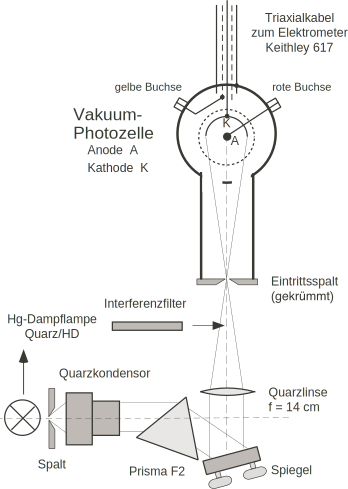
\includegraphics[width=0.45\textwidth]{experimental_arrangement_photoeffect}
	}
	\hfill
	\subfloat[Simplified schematic of the LED connections. A 10 $\Omega$ shunt is used to measure the current. The voltage is measured directly. \label{subfig:experimental_arrangement_led}]{
		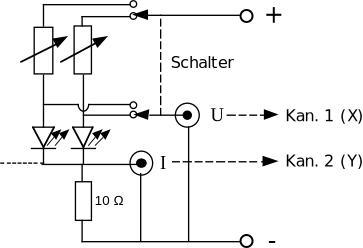
\includegraphics[width=0.45\textwidth]{experimental_arrangement_led}
	}
	\caption{Further diagrams for the conducted experiments. \textbf{(a)} shows the measuring procedure for measurements nr. 1 and 2. \textbf{(b)} shows a simplified schematic of how the LEDs are connected to power and to the oscilloscope in measurement nr. 3.}
	\label{fig:experimental_arrangement_diagram}
\end{figure}


\subsection{Software}
\label{subsec:Software}
All measurements are listed in appendix \ref{sec:Measurements}. The following software was used to record and evaluate the measurements:

\begin{itemize}
	\item Microsoft Office 365 Excel (64-bit)
	\item QtiPlot 0.9.9.2 (64-bit)
	\item Logger Pro 3.8.3 (64-bit)
\end{itemize}

% -------------------------------------------------------------------------------------------
\newpage
\subsection{Measurement Objects}
\label{subsec:measurement_objects}
The measurement objects are a mercury-vapor lamp and several different LEDs.

\paragraph{Mercury-Vapor Lamp}
Figure \ref{fig:hg} shows the spectrum of a mercury-vapor lamp which was measured.

\begin{figure}[H]
	\centering
	\includegraphics[width=\textwidth]{hg}
	\caption{The left picture shows the spectrum of a mercury-vapor lamp. A dispersive prism was used to disperse the light of the lamp. The right picture shows the line spectrum of a mercury-vapor lamp with the most important peaks annotated \cite{mercury-vapor_lamp_picture}. - partially modified}
	\label{fig:hg}
\end{figure}

The photoelectric voltage was measured at the following wave lengths shown in table \ref{tab:hg_colors}:

\begin{table}[H]
	\centering
	\renewcommand{\arraystretch}{1.2}
	\begin{tabular}{cc|c}
		\textbf{Wave length} $\lambda$ \cite{mercury-vapor_lamp} &  & \textbf{Color} \\
		\hline
		\textbf{365.4 nm} &  & Ultraviolet (UVA) \\
		\textbf{404.7 nm} &  & Violet \\
		\textbf{435.8 nm} &  & Blue \\
		\textbf{546.1 nm} & $^{1)}$ & Green \\
		\textbf{578.2 nm} & $^{2)}$ & Orange / Yellow \\ \hline
	\end{tabular}
	\caption{This table lists the wave length and their respective color.}
	\label{tab:hg_colors}
\end{table}

$^{1)}$ To measure the photoelectric voltage at a wavelength of 546.1 nm the filter OG530 was used.
$^{2)}$ To measure the photoelectric voltage at a wavelength of 578.2 nm the filter OG570 was used.

An annotated picture of the used filters can be found in appendix \ref{sec:filters}.

\paragraph{LEDs}
Table \ref{tab:leds} shows the designation of the LEDs that were measured and their respective colors:

\begin{table}[H]
	\centering
	\renewcommand{\arraystretch}{1.2}
	\begin{tabular}{r|l}
		\textbf{Designation} & \textbf{Color} \\
		\hline
		\textbf{L-7113QBC-D} & Blue \\
		\textbf{L-7113SGC} & Green \\
		\textbf{L-7113SYC-H} & Yellow \\
		\textbf{L-7113SEC-H} & Red \\
		\textbf{L-7114QWC-D} & White \\
		\textbf{LD 274} & Infrared \\ \hline
	\end{tabular}
	\caption{This table lists the wave length and their respective color.}
	\label{tab:leds}
\end{table}
